\documentclass[class=article, crop=false]{standalone}
\usepackage[fleqn]{amsmath}
\usepackage{amssymb}
\usepackage{mathtools}
\usepackage{graphicx}
\graphicspath{ {../images/} }
\begin{document}
\DeclarePairedDelimiter\abs{\lvert}{\rvert}%
\DeclarePairedDelimiter\norm{\lVert}{\rVert}%

\makeatletter
\let\oldabs\abs
\def\abs{\@ifstar{\oldabs}{\oldabs*}}

\let\oldnorm\norm
\def\norm{\@ifstar{\oldnorm}{\oldnorm*}}
\makeatother

\newcommand*{\Value}{\frac{1}{2}x^2}%


\section*{Idea}
\begin{itemize}
\item (physics) Linear displacement of objects. 
\item (maths) Do geometric algebra.
\item Two vectors are the same if they have the same direction and magnitude. 
\item Vectors represent directed line segments. 
\end{itemize}
\section*{Representation}
A vector of reals can be represented by $\mathbb{R}^n$ where n is the number of items in the vector.
\subsection*{Component representation:}
$ \vec{v} = \begin{bmatrix} v_1 \\ v_2 \\ \vdots \\ v_n \end{bmatrix} $\\
\subsection*{Basis representation:}
$ \vec{v} = v_1 \vec{e_1} + v_2 \vec{e_2} + \dots + v_n \vec{e_n} $ \\
In text book $\vec{e_1}, \vec{e_2}, \vec{e_3} $ etc. may be written as $\vec{i}, \vec{j}, \vec{k}$ \\
$\vec{e_n}$ represents a unit vector along one of the axes. E.g. in 2 dimensions, $\vec{e_2} = \begin{bmatrix} 0 \\ 1 \end{bmatrix} $
\subsection*{Polar representation:}
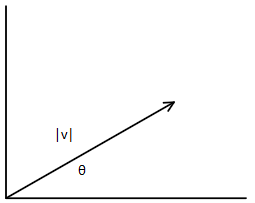
\includegraphics[scale=0.5]{fig1}\\
Where $ \vec{v} = \abs{\vec{v}} \begin{bmatrix} \sin \theta \\ \cos \theta\end{bmatrix} $
\section*{Operations}
\subsection*{Addition}
Vector addition is commutative (order doesn't matter) and associative (bracketing doesn't matter).
\subsection*{Example 1:}
\begin{align*}
\begin{bmatrix} p_1 \\ p_2 \end{bmatrix} + 
\begin{bmatrix} q_1 \\ q_2 \end{bmatrix} &= 
\begin{bmatrix} p_1 + q_1 \\ p_2 + q_2 \end{bmatrix} \\\\
\vec{u} + \vec{w} + \vec{v} & = \vec{u} + ( \vec{w} + \vec{v} ) \\
		  & = \vec{u} + ( \vec{v} + \vec{w} )
\end{align*}
\subsection*{Scalar Multiplication}
$ \lambda \vec{v} \qquad \lambda \in \mathbb{R}$\\
$\lambda$ Scales the vector but keeps the direction if positive, reverses if negative.\\
\subsection*{Example 2:}
\begin{align*}
\lambda \begin{bmatrix} v_1 \\ v_2 \\ \vdots \\ v_n \end{bmatrix} & = 
\begin{bmatrix} \lambda v_1 \\ \lambda v_2 \\ \vdots \\ \lambda v_n \end{bmatrix} \\\\ 
\abs{\lambda \vec{v}} & = \lambda \abs{\vec{v}} \\\\
\abs{\vec{v}} & = \sqrt{v_1^2 + v_2^2 \dots + v_n^2}
\end{align*}
What happens when $\lambda = 0$? We need to define a zero vector: 
\begin{align*}
\vec{o} & = 
\begin{bmatrix}
	0 \\
	0 \\
	\vdots \\
	0 \\
\end{bmatrix}
\end{align*}
Zero vector is the additive identity 
\subsection*{Scalar product}
Scalar product of $\vec{a}$,$\vec{b}$ is written $\vec{a} \cdot \vec{b}$ where:
\begin{align*}
\vec{a} & \cdot \vec{b} = \abs{\vec{a}} \abs{\vec{b}} \cos{\theta} \\ \therefore \mathbb{R}^n & \cdot \mathbb{R}^n \in \mathbb{R}
\end{align*}
and $\theta$ is the angle between the two vectors.\\
This has several interesting properties:\\
\begin{itemize}
	\item $\vec{a} \cdot \vec{a} = \abs{\vec{a}}^2$
	\item $\vec{a} \cdot \vec{b} = 0 \iff \vec{a} \perp \vec{b}$
	\item Dot product is commutative e.g. $\vec{a} \cdot \vec{b} = \vec{b} \cdot \vec{a}$
	\item $\vec{a}(\vec{b} + \vec{c}) = \vec{a} \cdot \vec{b} + \vec{a} \cdot \vec{c}$
	\item $(\lambda \vec{a}) \cdot (\mu \vec{b}) = \lambda \mu (\vec{a} \cdot \vec{b})$
\end{itemize} 
\begin{align*}
\text{If } \vec{a} & =
\begin{bmatrix}
a_1 \\ a_2 \\ \vdots \\ a_n \\
\end{bmatrix} \\
\vec{b} & =
\begin{bmatrix}
b_1 \\ b_2 \\ \vdots \\ b_n \\
\end{bmatrix} \\
\vec{a} \cdot \vec{b} & = (a_1 \vec{e_1} + a_2 \vec{e_2} + \dots + a_n \vec{e_n}) \cdot (b_1\vec{e_1} + b_2 \vec{e_2} + \dots + b_n \vec{e_n)} \\
& = a_1 \vec{e_1} \cdot b_1 \vec{e_1} + a_1 \vec{e_1} \cdot b_2 \vec{e_2} + \cdots + a_n\vec{e_n} \cdot b_n\vec{e_n} \;(n^2 \text{ terms}) \\
& = a_1b_1 + 0 + \dots + a_nb_n \; (\text{terms are 0 as }e_n \perp e_h \; h \neq n) \\
& = a_1b_1 + a_2b_2 + a_3b_3 + \dots + a_nb_n \\ 
\end{align*}
\subsection*{Example 3:}
Find the angle between $\begin{bmatrix} 3 \\ 5 \\ -2 \\ \end{bmatrix}$ and  $2\vec{e_1} - 3\vec{e_2}+\vec{e_3}$ \\
\begin{align*}
2\vec{e_1} - 3\vec{e_2}+\vec{e_3} &= \begin{bmatrix} 2 \\ -3 \\ 1 \\ \end{bmatrix}\\
\cos{\theta} &= 
\frac{
	\begin{bmatrix} 3 \\ 5 \\ -2 \\ \end{bmatrix} \cdot 
	\begin{bmatrix} 2 \\ -3 \\ 1 \\ \end{bmatrix}}
	{\abs{
		\begin{bmatrix} 3 \\ 5 \\ -2 \\ \end{bmatrix}} \cdot 
		\abs{\begin{bmatrix} 2 \\ -3 \\ 1 \\ \end{bmatrix}}} \\
& = \frac{-11}{\sqrt{3^2 + 5^2 + 2^2} \cdot \sqrt{2^2 + (-3)^2 + 1^2}} \\
& = \frac{-11}{2 \sqrt{133}} \\
\theta & = \arccos{\frac{-11}{2 \sqrt{133}}} = 118.5 \deg
\end{align*}
\section*{Vectors and coordinates}
Vector space is any type that the same algebraic rule as a vector (commutativity, associativity and distributivity).
\subsection*{How can we link vectors back to coordinates?}
A vector can represent the displacement from the origin of a point.
$ \vec{v} = \overrightarrow{OP} $ Represents the displacement of point P relative to the origin as we always need a frame of reference. This is called a position vector.
\section*{Applications of vectors}
We can use vectors to represent shapes with position vectors to vertices. From there you can then do calculations with the vectors.\\
They can also be used to represent positional and movement data. 
\subsection*{Example 3:}
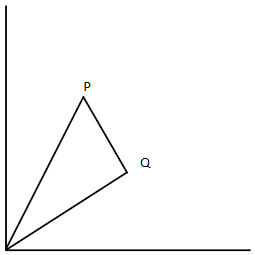
\includegraphics[scale=0.5]{fig2} \\
\begin{align*}
\overrightarrow{PQ} = \overrightarrow{OP} - \overrightarrow{OP}
\end{align*}
You can also use vectors to represent the equation of a line:
\begin{align*}
v & \in \mathbb{R}^n \\
\vec{x}: \mathbb{R} & \rightarrow \mathbb{R}^n \\
t & \mapsto \vec{v}t + \vec{x_0} \\
\end{align*}
\end{document}